\documentclass[
    letterpaper % use letter paper
]{article}

\includeonly{test1._include_,test4._include_}

\usepackage{graphicx}
\usepackage{nomencl}
\usepackage{hyperref}

\usepackage{apalike}\bibliographystyle{apalike}
%\usepackage{named}\bibliographystyle{named}

\makeglossary

\begin{document}

This is a nomenclature statement about NOMS.\nomenclature{NOMS}{Hello Nom Kitty}.

\tableofcontents
\listoffigures

\section{first section}

%\printglossary

\nocite{testentry3}

\begin{figure}
\centering
    \includegraphics[width=0.7\textwidth]{test1}
\caption{This is a figure}
\label{fig:test1}
\end{figure}

\section{second section}

\begin{figure}
\centering
    \includegraphics[width=0.7\textwidth]{test2}
\caption{This is another figure}
\label{fig:test2}
\end{figure}

\ref{fig:missing-and-very-long-to-push-errors-over-the-eol}

\begin{figure}
\centering
    \includegraphics[width=\textwidth]{graph}
\caption{This is another figure}
\label{fig:test3}
\end{figure}

\begin{figure}
\centering
    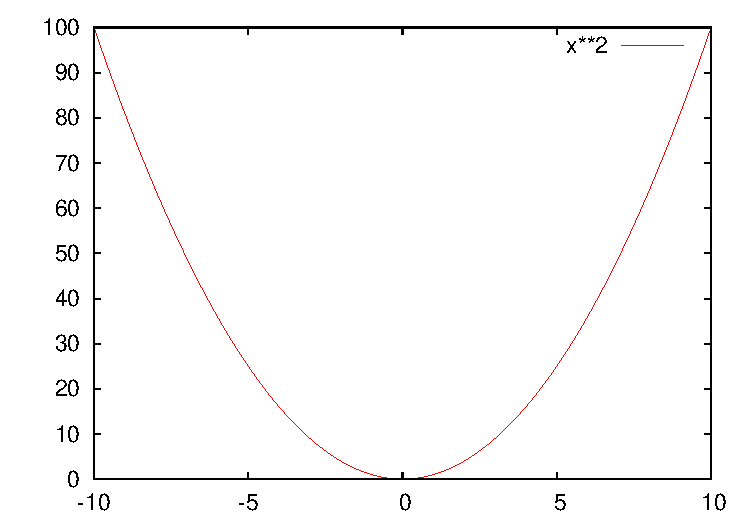
\includegraphics[width=\textwidth]{test4}
\caption{Test 4}
\label{fig:test4}
\end{figure}

A Citation: \cite{testentry}

This is an input: {This is test 3
}

This is test 1
\includegraphics[width=0.6\textwidth]{test3}

\cite{testentry2}
\cite{testentry4}
\bibliography{test-bib,test-bib2}

This is test 2


Now referring to Figures~\ref{fig:test1} and~\ref{fig:test2}.

\end{document}

% vim: lbr
